\documentclass[a0,portrait]{a0poster}
\renewcommand\refname{}
\usepackage{multicol}
\usepackage{subfloat}
\columnsep=100pt
\columnseprule=3pt
\let\chapter\section
\let\section\subsection
\let\subsection\subsubsection
\let\subsubsection\paragraph

\usepackage[svgnames]{xcolor}
\usepackage{tcolorbox}
\usepackage{graphicx}
\usepackage[font=large,labelfont=bf]{caption}
\usepackage{url}

\begin{document}
% Logo Its
\begin{minipage}[b]{0.25\linewidth}

\includegraphics[width=\linewidth]{logo-its}
\end{minipage}
\begin{minipage}[b]{0.75\linewidth}

% Judul
\veryHuge \color{NavyBlue} \textbf{Metode Pengaliran Data Audio melalui Sistem Penyeimbang Muat berbasis HAProxy} \\
\huge \color{black} \textbf{Putu Wiramaswara Widya \& Bahrul Halimi} \\
\Huge Jurusan Teknik Informatika \\
Institut Teknologi Sepuluh Nopember


\end{minipage}
\hline
\begin{multicols}{2}
\LARGE
\begin{tcolorbox}[colback=blue!5!white,colframe=blue!75!black,title=Pendahuluan]
Radio Internet adalah salah satu aplikasi Internet yang semakin banyak digunakan. Berbeda dengan radio konvensional yang mengirimkan suara dalam bentuk gelombang radio analog, radio Internet dikirimkan secara digital ke setiap penerima satu per satu menggunakan jaringan Internet berbasis TCP/IP. Dengan kata lain, semakin banyak suatu radio Internet maka semakin padat juga penggunaan jaringan dan beban server yang menyokongknya.

Dalam penelitian ini, dilakukan proses implementasi server radio Internet menggunakan teknik pembagi muat (\textbf{load balancer}) berbasis HAProxy. Perangkat lunak server radio Internet yang digunakan adalah IceCast yang berlisensi terbuka.
\end{tcolorbox}

\begin{tcolorbox}[colback=blue!5!white,colframe=red!75!black,title=Pengujian]
	Hasil pengujian dengan metode pengujian disamping menghasilkan data beragam. Di bawah ini data yang dihasilkan dari pengujian server yang diakses tanpa melalui load balancer.
	\ \\
	\begin{center}
		\begin{tabular}{|c|c|c|}
			\hline
			\textbf{Pengakses} & \textbf{Terpenuhi} & \textbf{Gagal} \\ \hline
			90 & 90 & 0 \\ \hline
			150 & 150 & 0 \\ \hline
			300 & 300 & 0 \\ \hline
			450 & 346 & 104 \\ \hline
			600 & 243 & 357 \\ \hline
		\end{tabular}
	\end{center}
	\ \\
	Sementara itu, berikut data yang dihasilkan dari pengujian akses melalui load balancer.	
	\ \\
	
	% Diakses melalui HAProxy
	\begin{center}
		\begin{tabular}{|c|c|c|}
			\hline
			\textbf{Pengakses} & \textbf{Terpenuhi} & \textbf{Gagal} \\ \hline
			90 & 90 & 0 \\ \hline
			150 & 150 & 0 \\ \hline
			300 & 300 & 0 \\ \hline
			450 & 434 & 16 \\ \hline
			600 & 485 & 115 \\ \hline
		\end{tabular}
	\end{center}
	
	\ \\
	\textbf{\underline{Analisis}.} Pengujian dengan klien berjumlah 90, 150, dan 300 memiliki tingkat keberhasilan 100\% dan tingkat kegagalan 0\%. Angka ini berubah ketika jumlah pengakses ditingkatkan. Pada saat klien berjumlah 450, tingkat keberhasilan 76,8\% dan tingkat kegagalan 23.2\% untuk akses tanpa load balancer. Sementara itu untuk akses melalui load balancer memberikan tingkat keberhasilan 96,4\% dan tingkat kegagalan 3,6\% dengan jumlah pengakses yang sama. Perbadaan keberhasilan dan kegagalan ini juga terjadi ketika terdapat 600 pengakses dalam waktu yang hampir bersamaan.
		
		
\end{tcolorbox}

\begin{tcolorbox}[colback=blue!5!white,colframe=green!75!black,title=Metode]
	\textbf{\underline{Permasalahan}.} Bagaimana menyeimbangkan muatan kerja server yang	menyiarkan audio ke pendengar ketika ada banyak permintaan secara bersamaan? Bagaimana menyediakan banyak server untuk melayani permintaan pendengar dengan satu sumber aliran dari pengirim?
	
	\begin{center}
		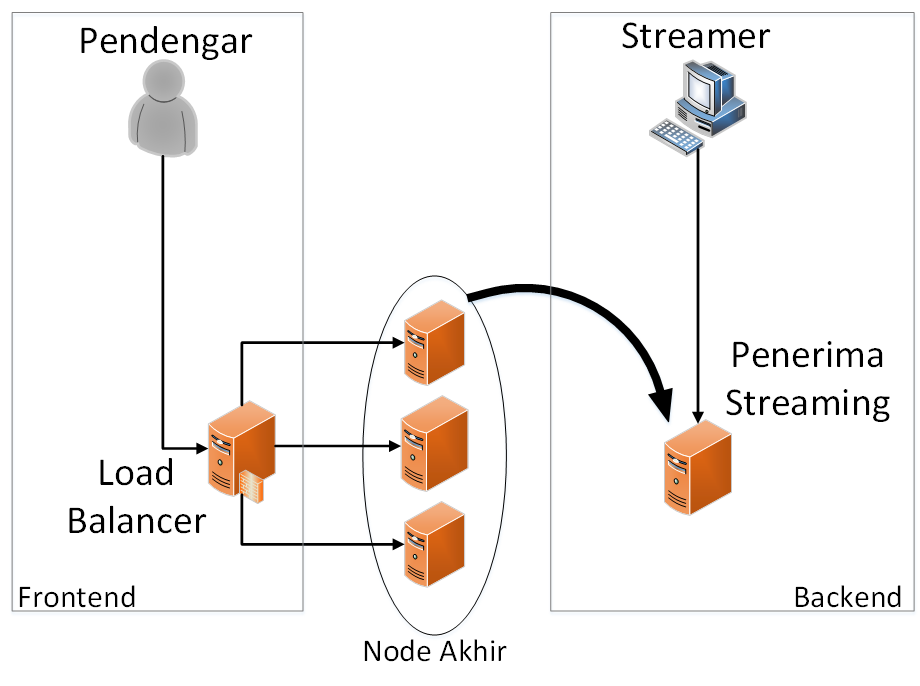
\includegraphics[width=0.7\linewidth]{arsitektur}
	\end{center}

	\textbf{\underline{Arsitektur Jaringan}.} Terdapat tiga server radio Internet yang nantinya akan digunakan dengan metode penyeimbang muat, satu server utama di bagian \textbf{Frontend\textit{}}, dan satu server utama di bagian \textbf{Backend\textit{}}. Server utama di bagian Frontend berhadapan dengan pendengar, sedangkan server utama di bagian Backend berhadapan dengan pengirim.
	
	\ \\
	\textbf{\underline{Pengujian}.} Dua mekanisme disiapkan yaitu akses melalui load balancer dan akses tanpa load balancer. Perhitungan dilakukan dengan melakukan uji \texttt{stress test} pada load balancer atau langsung ke server radio Internet. Akses dilakukan melalui tiga komputer penguji beban dengan jumlah klien yang disimulasikan adalah 90,150,300,450, dan 600.
	


\end{tcolorbox}


\begin{tcolorbox}[colback=blue!5!white,colframe=blue!75!black,title=Referensi,fontupper=\normalsize]

	\begin{thebibliography}{9}
		\bibitem{setupice}
		Xiph.Org
		\textbf{Icecast 2.4.1 Docs — Basic Setup},[Online],
		\url{http://icecast.org/docs/icecast-2.4.1/basic-setup.html},
		diakses tanggal 23 Desember 2014
		\bibitem{ice}
		Xiph.Org
		\textbf{Icecast is free server software for streaming multimedia},[Online],
		\url{http://icecast.org/},
		diakses tanggal 1 September 2014
		\bibitem{halebih}
		Mark Imbriaco
		\textbf{Nuts \& Bolts: HAproxy},[Online],
		\url{https://signalvnoise.com/posts/1073-nuts-bolts-haproxy},
		diakses tanggal 1 September 2014
		\bibitem{haproxy}
		HAProxy
		\textbf{Description},[Online],
		\url{http://www.haproxy.org/#desc},
		diakses tanggal 1 September 2014
		\bibitem{hause}
		HAProxy
		\textbf{They use it !},[Online],
		\url{http://www.haproxy.org/they-use-it.html},
		diakses 1 September 2014
		\bibitem{nodejs}
		Joyent, Inc
		\textbf{Node.js v0.10.35 Manual \& Documentation},[Online],
		\url{http://nodejs.org/api/stream.html},
		diakses tanggal 23 Desember 2014
		\bibitem{nodejsieee}
		Stefan Tilkov, Steve Vinoski,
		\textbf{Node.js: Using JavaScript to Build High-Perfomace Network Programs},
		IEEE Computer Society Issue 06, Nov-Dec 2010,
		pp 80-83, 2010
		
	\end{thebibliography}
	
\end{tcolorbox}





\end{multicols}

\LARGE
\begin{tcolorbox}[colback=blue!5!white,colframe=red!75!white,title= ]
	
	
\includegraphics[width=0.25\linewidth]{logo-haproxy}	\hfill
	
\includegraphics[width=0.25\linewidth]{logo-nodejs} \hfill
	
\includegraphics[width=0.25\linewidth]{logo-icecast}
	
\end{tcolorbox}




\end{document}
